\documentclass{beamer}
%Information to be included in the title page:
\title{Piecewise Linear Function}
\subtitle{with discontinuity at $x = 0$}
\author{Fabian Weik}
\institute{Overleaf}
\date{\today}

\usepackage{listings}

\begin{document}

\frame{\titlepage}

\begin{frame}[fragile]{Code}
    \begin{lstlisting}
real_t x = currentState[0];
real_t y = 0;

if (x < 0) {
    y = aL * x + muL;
} else {
    y = aR * x + muR;
}

RHS[0] = y;
return true;
    \end{lstlisting}
    
    Executed using AnT
    
\end{frame}

\begin{frame}
\frametitle{2D Scan}
    Varying $\mu_L$ and $\mu_R$
    
    \centering
    \vspace*{1em}
    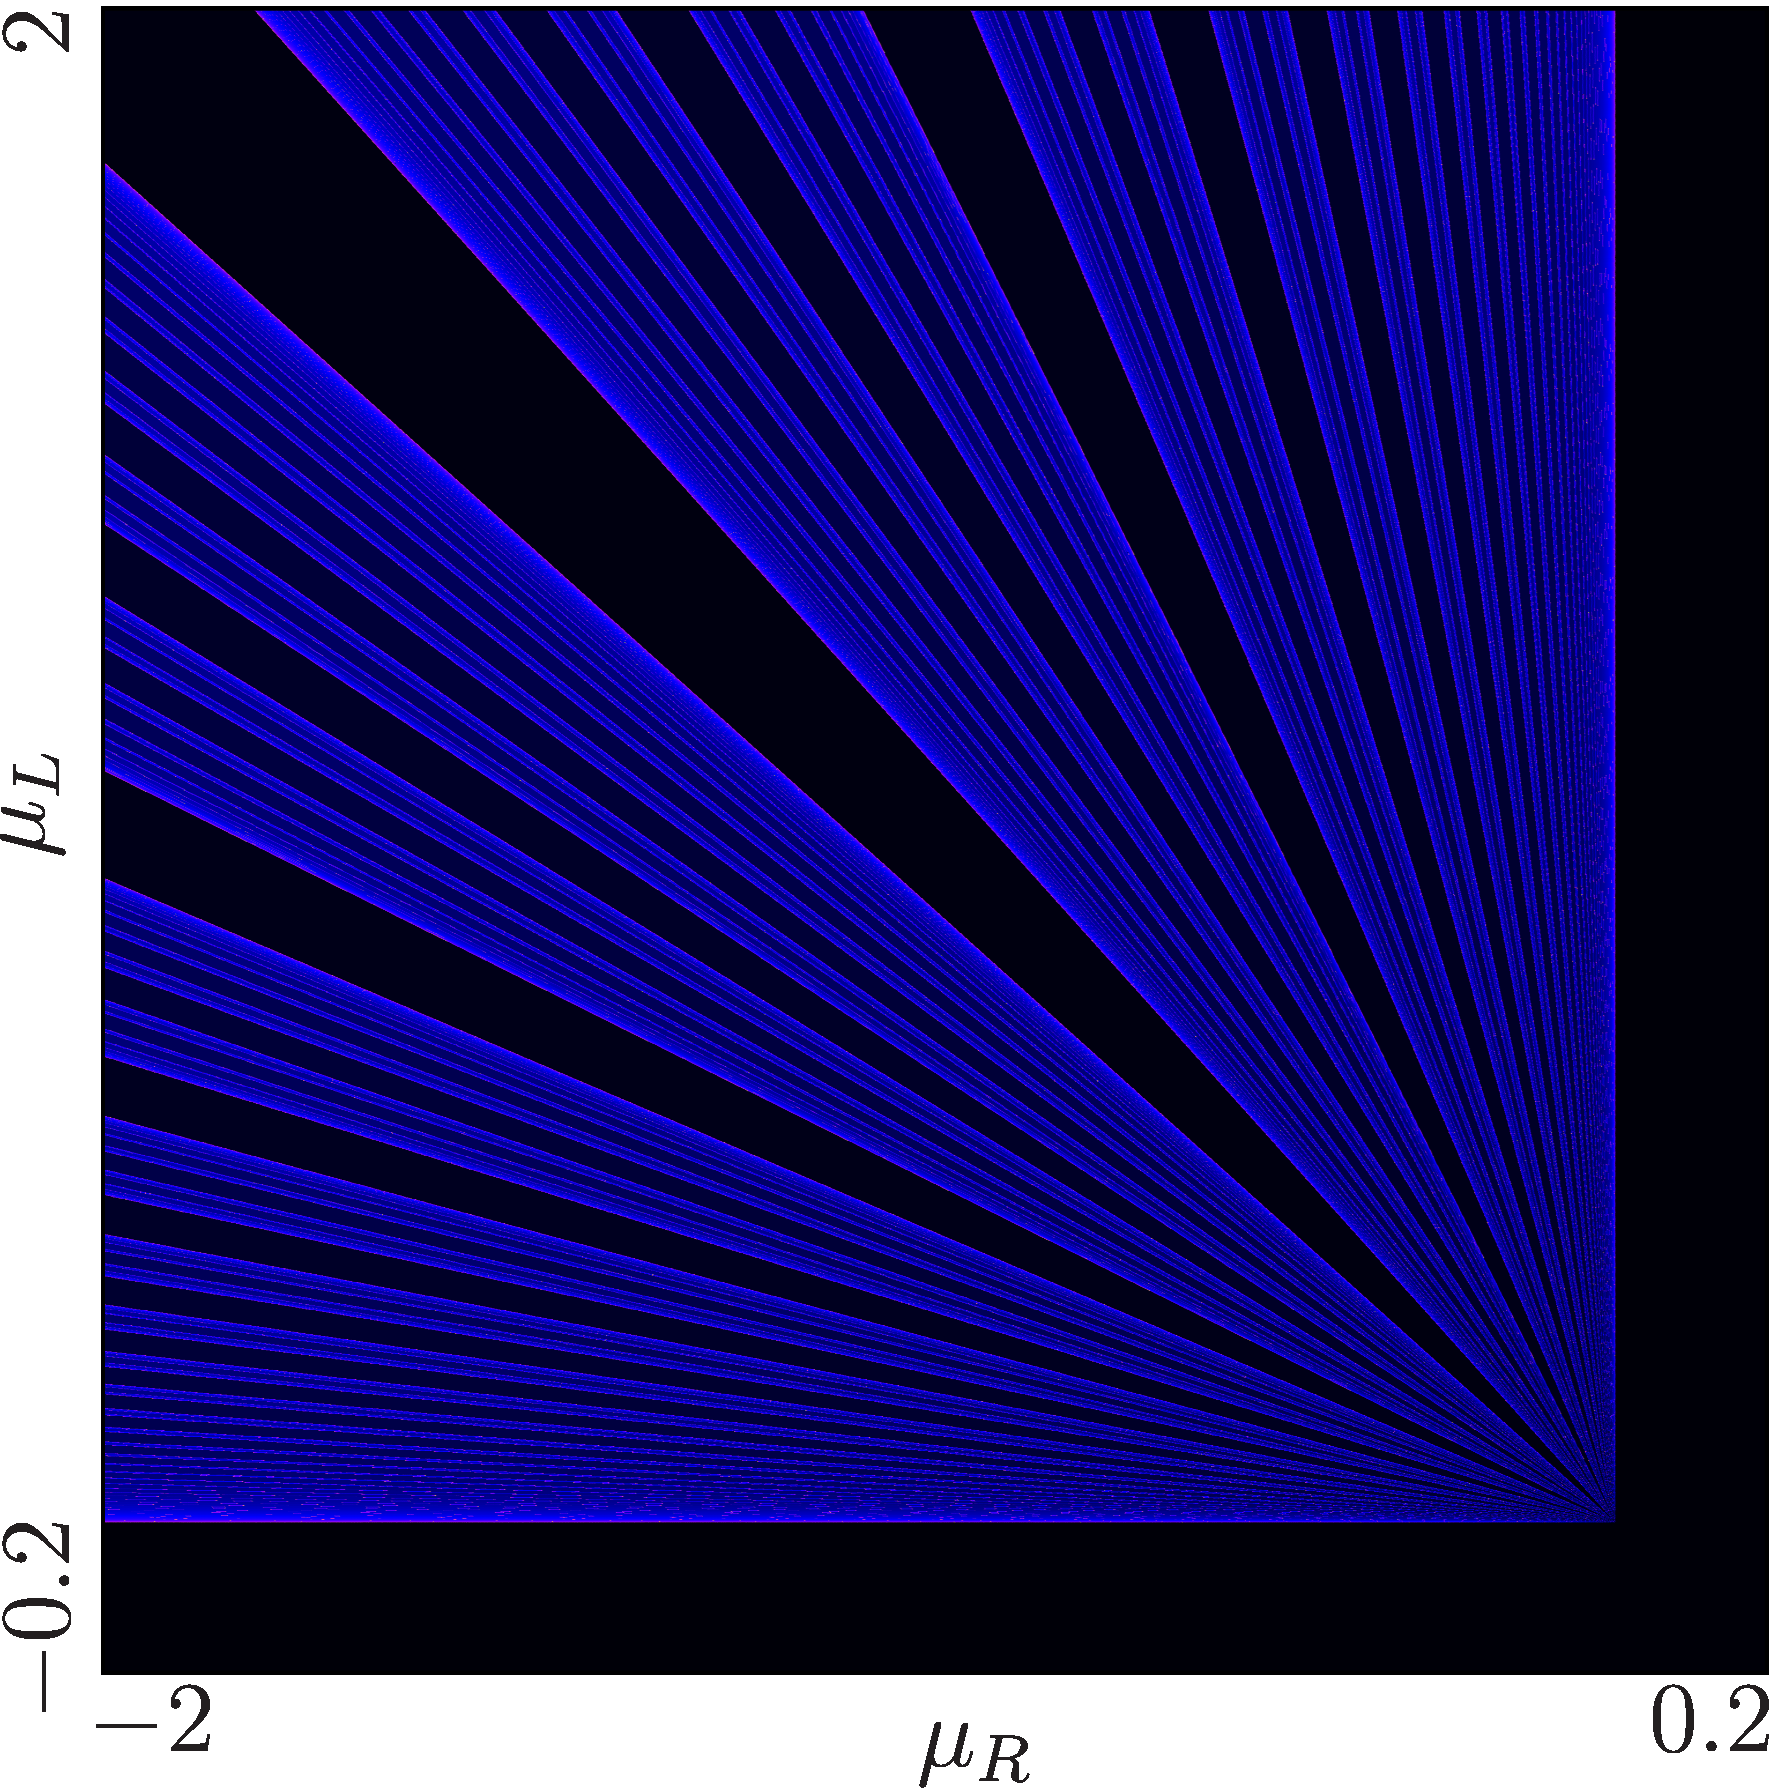
\includegraphics[width=0.6 \textwidth]{../../Simulation/Models/00_Examples/03_Homework_0110/2D_Period/result.png}
\end{frame}

\end{document}
